\documentclass[tikz,border=5pt]{standalone}
\usepackage{pgfplots}
\pgfplotsset{compat=1.18}

\begin{document}
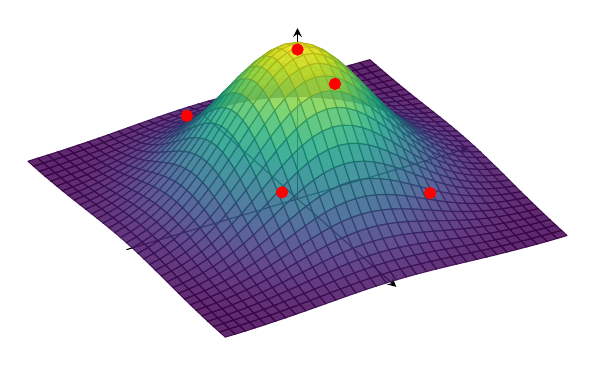
\begin{tikzpicture}
  \begin{axis}[
      view={60}{50},
      axis lines=middle,
    %   xlabel={$x$},
    %   ylabel={$y$},
    %   zlabel={$f(x,y)$},
      xmin=-2, xmax=2,
      ymin=-2, ymax=2,
      zmin=0,  zmax=1.2,
      xtick=\empty,
      ytick=\empty,
      ztick=\empty,
      colormap/viridis,
      samples=35,
      domain=-2:2,
      y domain=-2:2
    ]

    % 平滑“地形”：一个二维高斯凸起，可以理解为 RBF kernel 拟合后的表面
    \addplot3[
      surf,
      opacity=0.85,
    ]
    {1.06* exp(- (x^2 + y^2) / 1.3)};

    % 观测样本点（测得的海拔），大致贴在曲面上
    \addplot3[
      only marks,
      mark=*,
      mark size=2.0pt,
      color=red
    ]
    coordinates {
      (-1.2, -0.6, 0.32)
      (-0.8,  0.9, 0.40)
      ( 0.0,  0.0, 1.05)
      ( 0.9, -0.7, 0.45)
      ( 1.3,  0.8, 0.30)
    };

    % 给样本点加一点注释（可删）
    % \addplot3[->, thick]
    % coordinates {(0,0,1.15) (0,0,1.05)};
    % \node at (axis cs:0,0,1.2) {\small observed peak};

  \end{axis}
\end{tikzpicture}
\end{document}